\documentclass[11pt]{article}
\usepackage{amsmath,textcomp,amssymb,geometry,graphicx,enumerate}
\usepackage[T5]{fontenc}
\usepackage[utf8]{inputenc}

\def\Name{Quoc Thai Nguyen Truong}  % Your name
\def\SID{24547327}  % Your student ID number
\def\Login{cs170-ig} % Your login (your class account, cs170-xy)
\def\Homework{10}%Number of Homework
\def\Session{Fall 2014}


\title{CS170--Fall 2014 --- Solutions to Homework \Homework}
\author{\Name, SID \SID, \texttt{\Login}}
\markboth{CS170--\Session\  Homework \Homework\ \Name}{CS170--\Session\ Homework \Homework\ \Name, \texttt{\Login}}
\pagestyle{myheadings}

\newenvironment{qparts}{\begin{enumerate}[{(}a{)}]}{\end{enumerate}}
\def\endproofmark{$\Box$}
\newenvironment{proof}{\par{\bf Proof}:}{\endproofmark\smallskip}

\textheight=9in
\textwidth=6.5in
\topmargin=-.75in
\oddsidemargin=0.25in
\evensidemargin=0.25in


\begin{document}
\maketitle

\noindent
Collaborators: Hriday Kemburu, Kiet Lam


\section*{1. Linear programming practice}
\noindent
\textbf{Linear program.}
YOUR ANSWER GOES HERE

% The following Latex environment might be handy:
 \begin{align*}
 0 &\le x \le 40\\
 0 &\le y \le 30\\
 0 &\le z \le 20\\
 x + y + z  &\le 60\\
 2x + y  + 3z &\le 100\\
 max\{ 1000x + 1,200y + 12,000z \}
 \end{align*}
% (remove the percent signs at the start of the lines above)

\noindent
\textbf{List of variables and their meaning.}\\
$x:$ number of Xantalum cubic meters.\\
$y:$ number of Ytterbium cubic meters.\\
$z:$ number of Zastatine cubic meters.


\newpage
\section*{2. Henron}
\begin{qparts}
\item 
\textbf{Solution.}
In order to formulate this as a network flow problem, we need to have vertices and edges. there are two types of vertices: supplier and purchasers. Each supplier will represent a vertex, and each purchaser will represent a vertex. The edges will be a connection between supplier vertices and purchaser vertices in list of L , the value of theses edges are infinity. Create a vertex call $S$ and connect it to every supplier vertices and the value of these edges are $s[i]$ (supplier i). Create a vertex call $T$ and connect it to every purchaser vertices and the value of these edges are $b[j]$ (purchaser j). Now, we have a network flow, running Edmonds – Karp algorithm to get the max flow of the network which give us the maximum number of chickens that can be sold this year.
\\
\textbf{Graph.}
% You can include a picture using the following:
   \begin{center}
   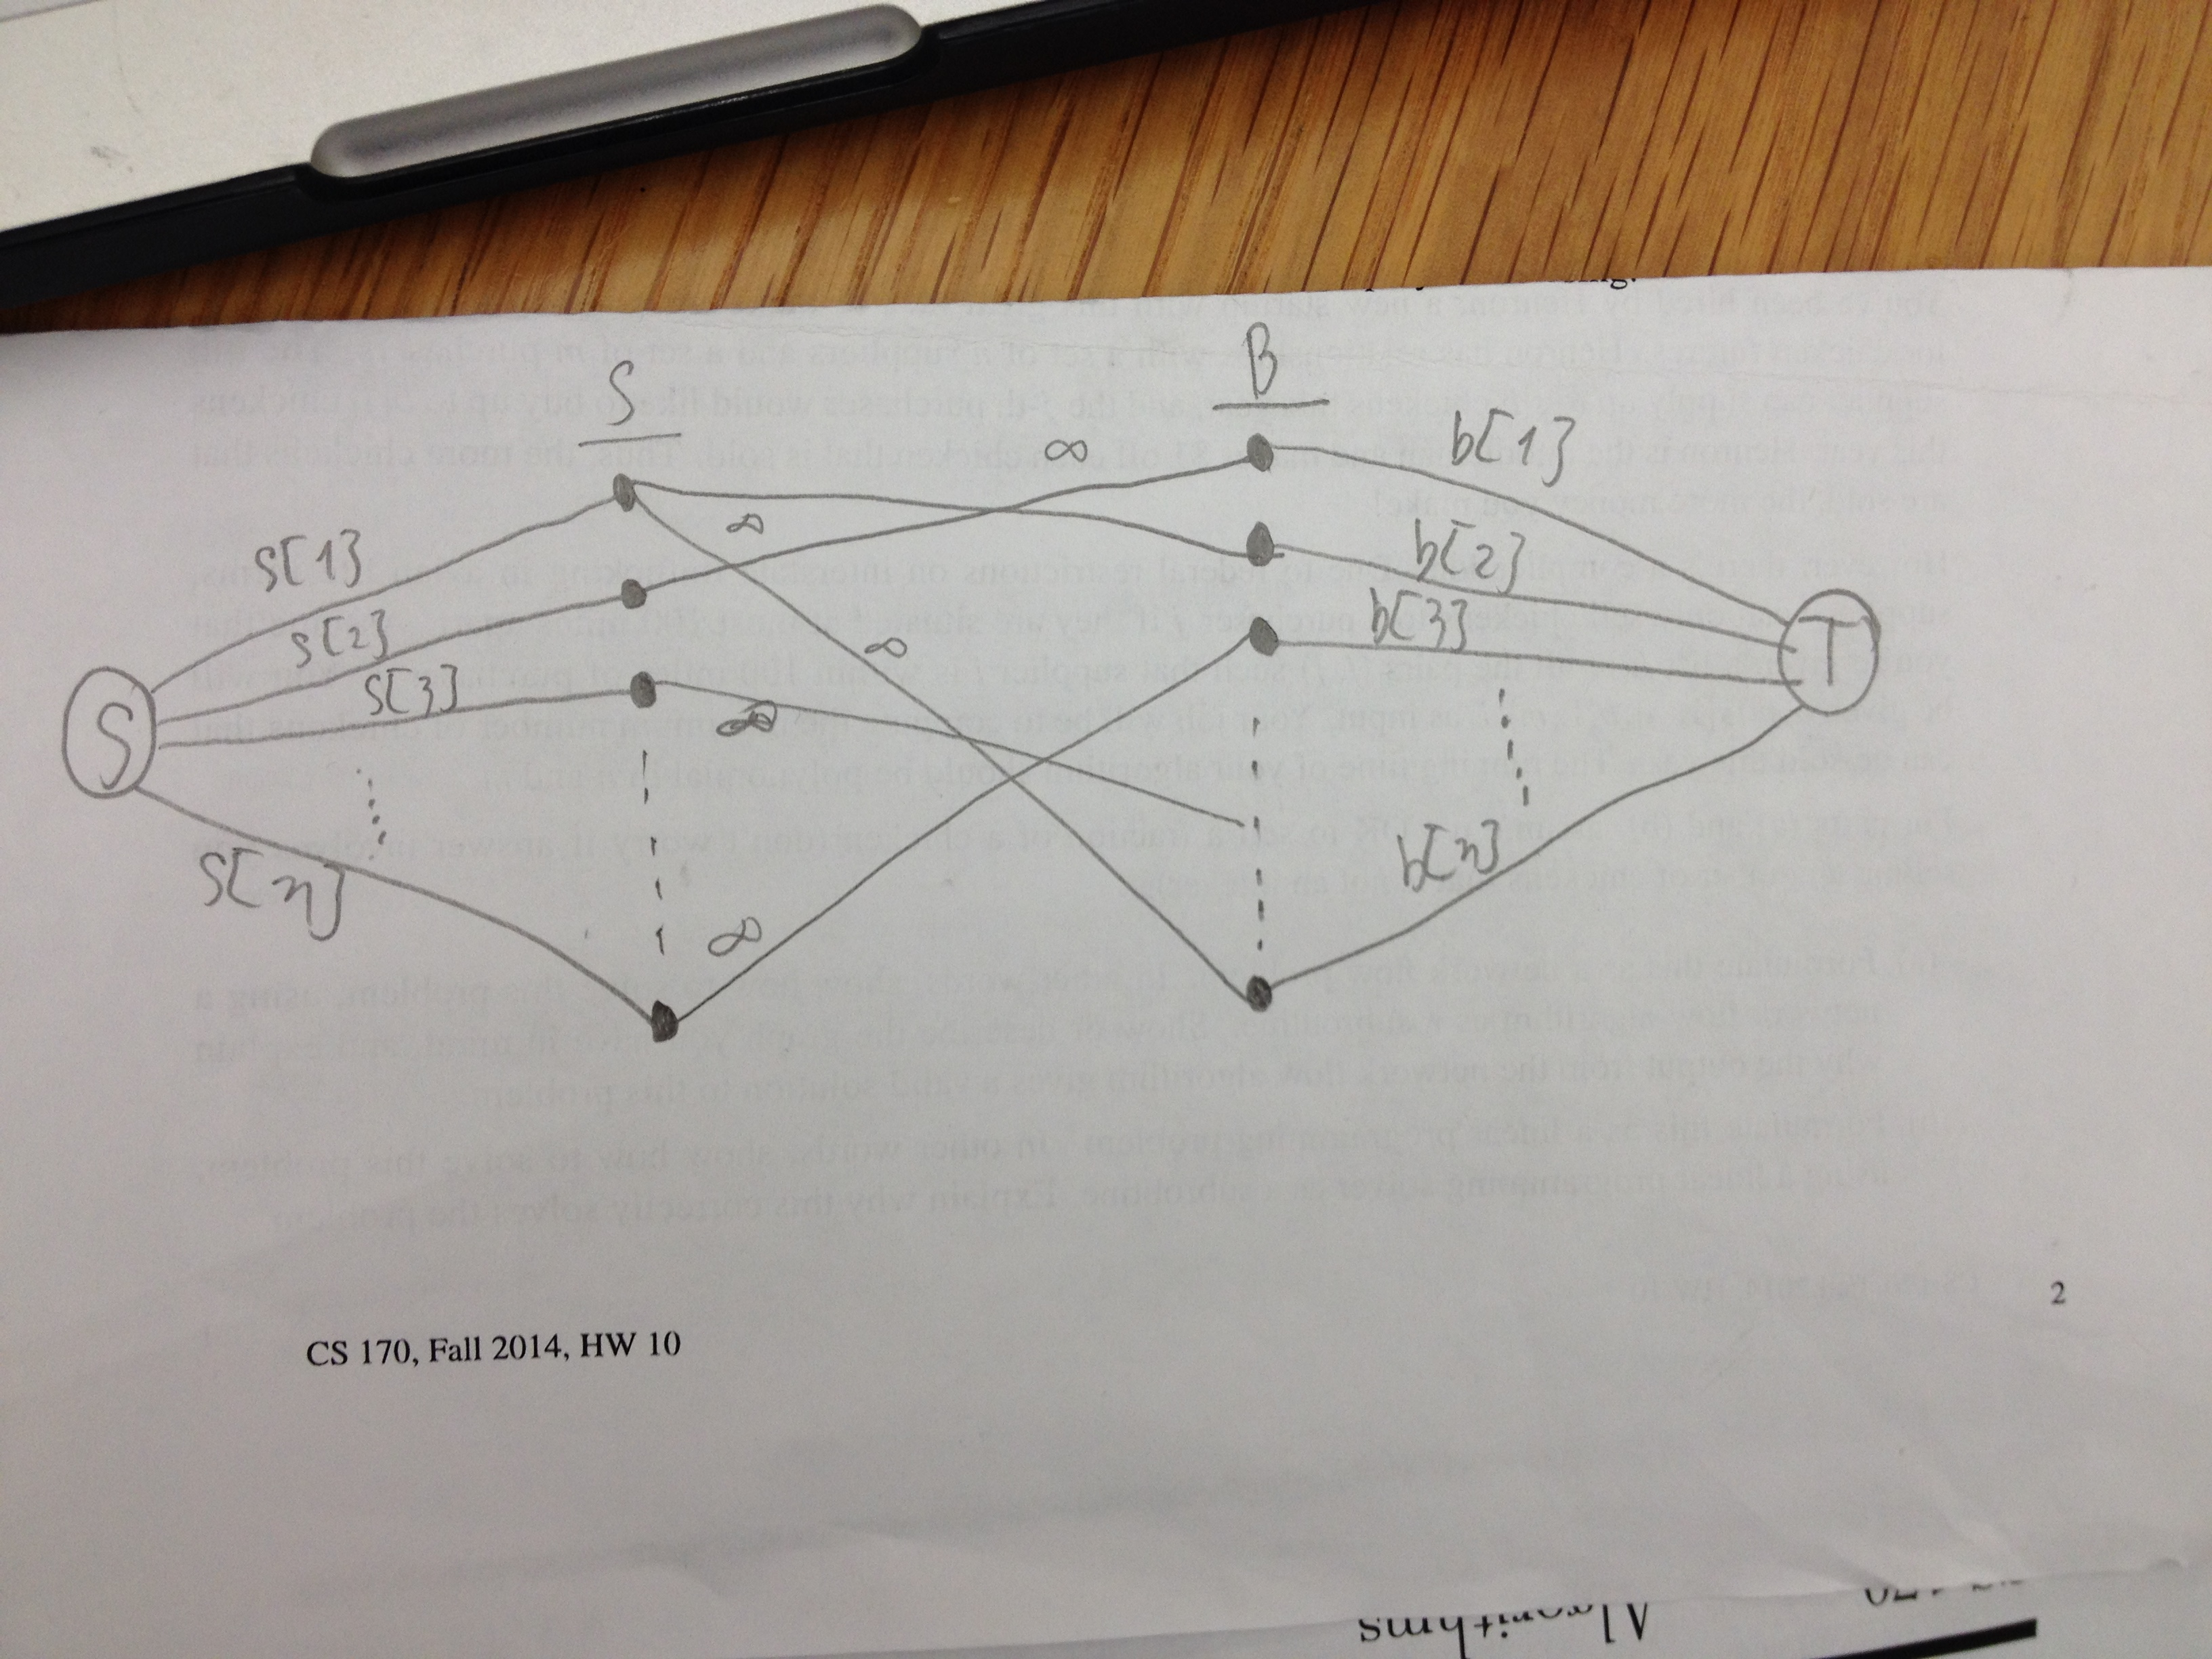
\includegraphics[scale=0.1]{p2a.JPG}
   \end{center}
% (remove the percent signs at the start of the lines above)
% you can also use a .png image, but other file formats are alas
% not supported by Latex.
\textbf{Justification.}\\
We have a source S, and all the edge connect to this source S have the value of the number of chickens that a seller can sell up to. We also have a sink T, and all the edge connect to this sink T have the value of the number of chickens that a buyer can buy up to. Make connections for each pair in list L(i,j) between seller i and buyer j. Now we can see that this is a network flow graph, the flow represent number of chickens. Using Edmonds Karp algorithm for this graph give us a maximum flow. Hence, in this maximum flow graph, the sum of number of chickens can be sell by all sellers equals to the sum of number of chickens can sell to all the buyer. Therefore, the sum is the maximum number of chickens can be sold this year. 
\item
\textbf{Solution.}\\
we can reduce this network flow problem to linear programming problem. We assign value to each edge in the network that will satisfy a set of linear constraints and maximize a linear object function. 
\\
Let $a_{i,j}$ = the transaction number of chickens between seller i and buyer j, $(i,j) \in L $.\\
Let $a_{s,i}$ = the transaction number of chickens between seller i and node s.\\
Let $a_{t,j}$ = the transaction number of chickens between purchaser j and node t.\\
$$a_{s,i} \leq s[i], 1 \leq i \leq n$$
$$a_{t,j} \leq b[j], 1 \leq j \leq m$$
$$a_{i,j} \geq 0$$
$$Max\ of \sum_{(i,j) \in L } a_{i,j}$$

\textbf{Justification.}\\
The number of variables are the number of edges in the network graph. There are 4 types of constraints: value of variables ($f$) has to be greater or equal to zero (can't have negative chickens), value of each edge (supplier i) coming out from $S$ has to be less than or equal to the number of  chickens that supplier i can supply up to s[i], value of each edge (purchaser j) coming in to $T$ has to be less than or equal to the number of chickens that the j purchaser j can buy up to b[j], and flow conservation (ex.$f_{s1,b2} + f_{s3,b2} = f_{b2,T}$).
And we maximum sum of all transactions number of chickens between seller i and buyer j (edge(i,j) $\in$ L) which give the maximum number of chickens that can be sold this year.\\

\item
\textbf{Which is better.}\\
\boxed{network\ flow} would be better 

\textbf{Explanation.}\\
Because the running for solving network  flow would be polynomial time compare to exponential run time for solving integer linear programming.\\ 

\end{qparts}

\newpage
\section*{3. 4-coloring}
\begin{qparts}
\item
\textbf{Reduction.}\\
We will reduce a graph G into a new graph G' , graph G is 3-coloring if and only if G' is 4-coloring. The way to turn G into G' is to set G' to G and create a node $S$ and connect it to every vertices in G'.\\
\\
\textbf{Proof of correctness.}\\
If graph G is 3-coloring, and we know that G' is 4-coring exactly like G with an extra node $S$ has only a color which is different than other vertices's color.\\
Same thing, if graph G' is 4-coloring, then we know that S is the only node of its color because it's connected to every other node in G'. Therefore, G must be 3-coloring.

\item
We can see that the reduction takes linear time to add a single node. We know how to solve a 4-coloring problem in polynomial time. Given the input is 3-coloring graph, add a single node (with a different color than other 3 colors of the graph) and connect it to every other nodes in the 3-coloring graph. Now we have a 4-coloring, solving it take polynomial time. Hence, the total run time is polynomial plus linear time which equivalent to polynomial time. Therefore, if there is a polynomial-time algorithm for the 4-coloring problem, then there is a polynomial-time algorithm for 3-coloring.
\end{qparts}

\newpage
\section*{4. Optional bonus problem}
YOUR ANSWER GOES HERE, if you want to answer it

\end{document}
